\documentclass[twoside]{article}
\usepackage[a4paper]{geometry}
\geometry{verbose,tmargin=2.5cm,bmargin=2cm,lmargin=2cm,rmargin=2cm}
\usepackage{fancyhdr}
\pagestyle{fancy}

% nastavení pisma a češtiny
\usepackage{lmodern}
\usepackage[T1]{fontenc}
\usepackage[utf8]{inputenc}
\usepackage[czech]{babel}

% odkazy
\usepackage{url}

\usepackage{float}
% vícesloupcové tabulky
\usepackage{multirow}
\usepackage{amssymb}
\usepackage{bbold}
\usepackage{amsmath}
\usepackage{mathtools}
\usepackage{commath}

% vnořené popisky obrázků
\usepackage{subcaption}

% automatická konverze EPS 
\usepackage{graphicx} 
\usepackage{epstopdf}
\epstopdfsetup{update}

\graphicspath{{./images}}

% odkazy a záložky
\usepackage[unicode=true, bookmarks=true,bookmarksnumbered=true,
bookmarksopen=false, breaklinks=false,pdfborder={0 0 0},
pdfpagemode=UseNone,backref=false,colorlinks=true] {hyperref}

% Poznámky při překladu
\usepackage{xkeyval}	% Inline todonotes
\usepackage[textsize = footnotesize]{todonotes}
\presetkeys{todonotes}{inline}{}

%https://tex.stackexchange.com/questions/2783/bold-calligraphic-typeface
\DeclareMathAlphabet\mathbfcal{OMS}{cmsy}{b}{n}

% Zacni sekci slovem ukol
\renewcommand{\thesection}{Úkol \arabic{section}}
% enumerate zacina s pismenem
\renewcommand{\theenumi}{\alph{enumi}}

% smaz aktualni page layout
\fancyhf{}
% zahlavi
\usepackage{titling}
\fancyhf[HC]{\thetitle}
\fancyhf[HLE,HRO]{\theauthor}
\fancyhf[HRE,HLO]{\today}
 %zapati
\fancyhf[FLE,FRO]{\thepage}

% údaje o autorovi
\title{Automatické řízení: DÚ 3 - Identifikace}
\author{Vojtěch Michal}
\date{\today}

\begin{document}

\maketitle

% ---------------------------------
% ---------------------------------
% název sekce je generován automaticky jako: Úkol X

\newcommand{\rad}{{rad}}
\renewcommand{\norm}{{norm}}
\renewcommand{\tan}{{tan}}

\section{Odezva systému prvního řádu}
Pokuste se identifikovat model prvního řádu. Výstup systému je zatížen šumem. Přenosovou funkci
modelu hledejte ve tvaru
\begin{equation}
	\label{eq:obecne1}
	F(s) = \frac{k}{Ts + 1}.
\end{equation}
Uveďte parametry identifikovaného systému, tj. zesílení $k$ a časovou konstantu $T$, získané identifikací a
krátký popis, jak jste při identifikaci postupovali, 
dále obrázek obsahující originální odezvu a odezvu matematického modelu, který jste získali identifikací. \\
\textbf{Řešení:} Změřený časový průběh odezvy systému na jednotkový skok je zobrazen na obrázku \ref{fig:zadani1}
v podobě syrových dat bez filtrace i po filtraci klouzavým průměrem délky tři vzorky, aby nedošlo ke znatelné deformaci odezvy.
I bez bližší analýzy je zjevné, že časová konstanta bude vysoká (korespondující pól bude pomalý), protože časová osa
přechodového děje trvá desítky vteřin. 
\begin{figure}[htbp]
	\centering
	\begin{subfigure}{0.45\textwidth}
		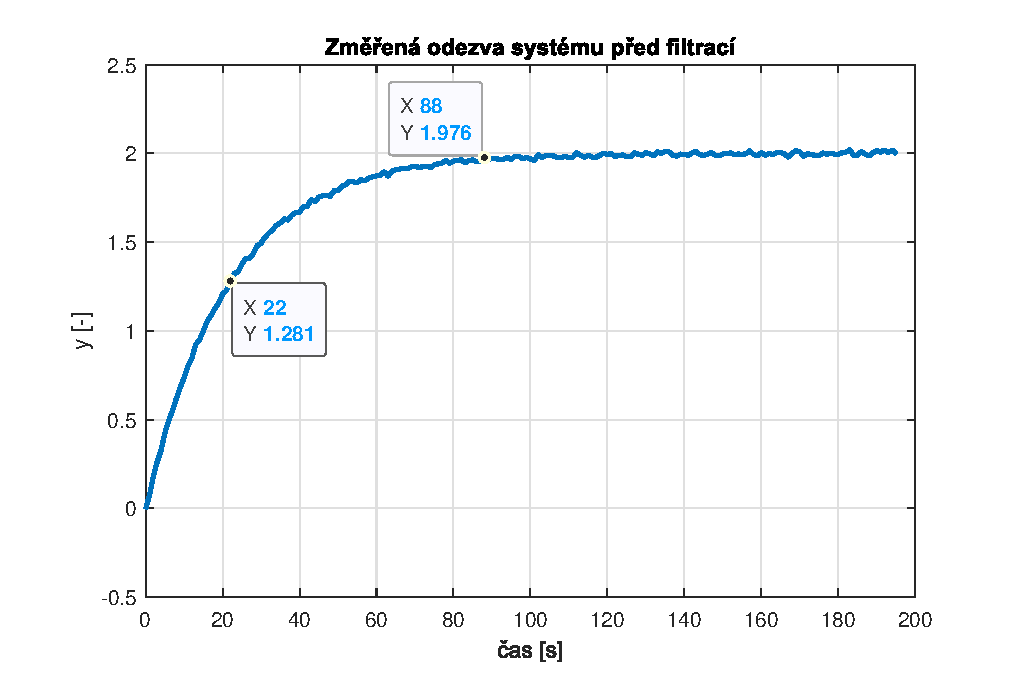
\includegraphics[width=\linewidth]{odezva1_raw.eps}
		\caption{Změřený průběh odezvy}
	\end{subfigure}
	\begin{subfigure}{0.45\textwidth}
		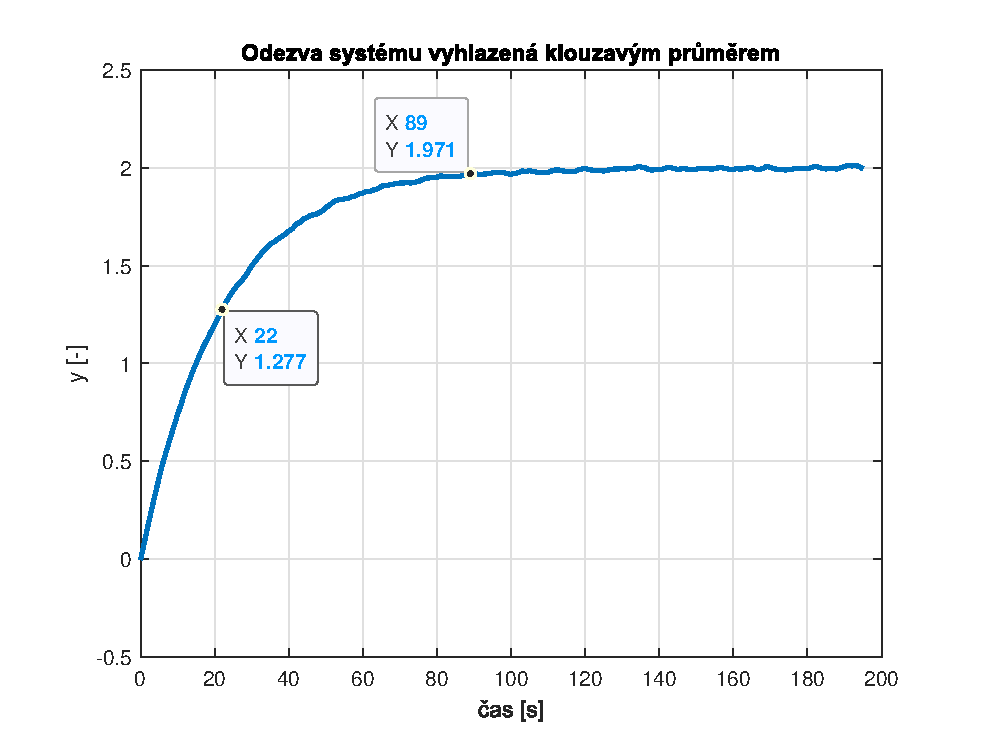
\includegraphics[width=\linewidth]{odezva1_filtered.eps}
		\caption{Průběh odezvy po filtraci}
	\end{subfigure}
	\caption{Časový průběh k identifikaci}
	\label{fig:zadani1}
\end{figure}

Statické zesílení systému je $k = 2$, k této hodnotě konvergují s rostoucím časem filtrovaná i nefiltrovaná odezva systému.
Dále je pro odezvu systému prvního řádu důležitý okamžik uplynutí jedné časové konstanty $t_1 = T$. Tehdy je magnituda
odezvy na jednotkový skok na hladině 63\% ustálené hodnoty. Nalezením času, ve kterém protíná odezva systému
úroveň $y = 0.63 \cdot 2 = 1.26$, nalezneme i časovou konstantu $T = 22$ s. Pro kontrolu je možné ověřit, 
že v čase $t_2 \approx 4T$ je odchylka odezvy od ustálené hodnoty menší než dvě procenta, což obrázek \ref{fig:zadani1} potvrzuje.

Dosazením odečtených konstant do obecného tvaru \eqref{eq:obecne1} získáme matematický model přenosu systému 
\begin{equation}
	F(s) = \frac{2}{22s + 1},
\end{equation}
jehož odezva na jednotkový skok je porovnána s měřenými daty na obrázku \ref{fig:zaver1}. Odezva modelu
věrně kopíruje změřenou odezvu systému, identifikace proběhla velice přesně. Protože se obě charakteristiky shodují
v čase blízkém nule, byl identifikovaný systém zřejmě opravdu řádu jedna a byl bez nul.
\begin{figure}
	\centering
	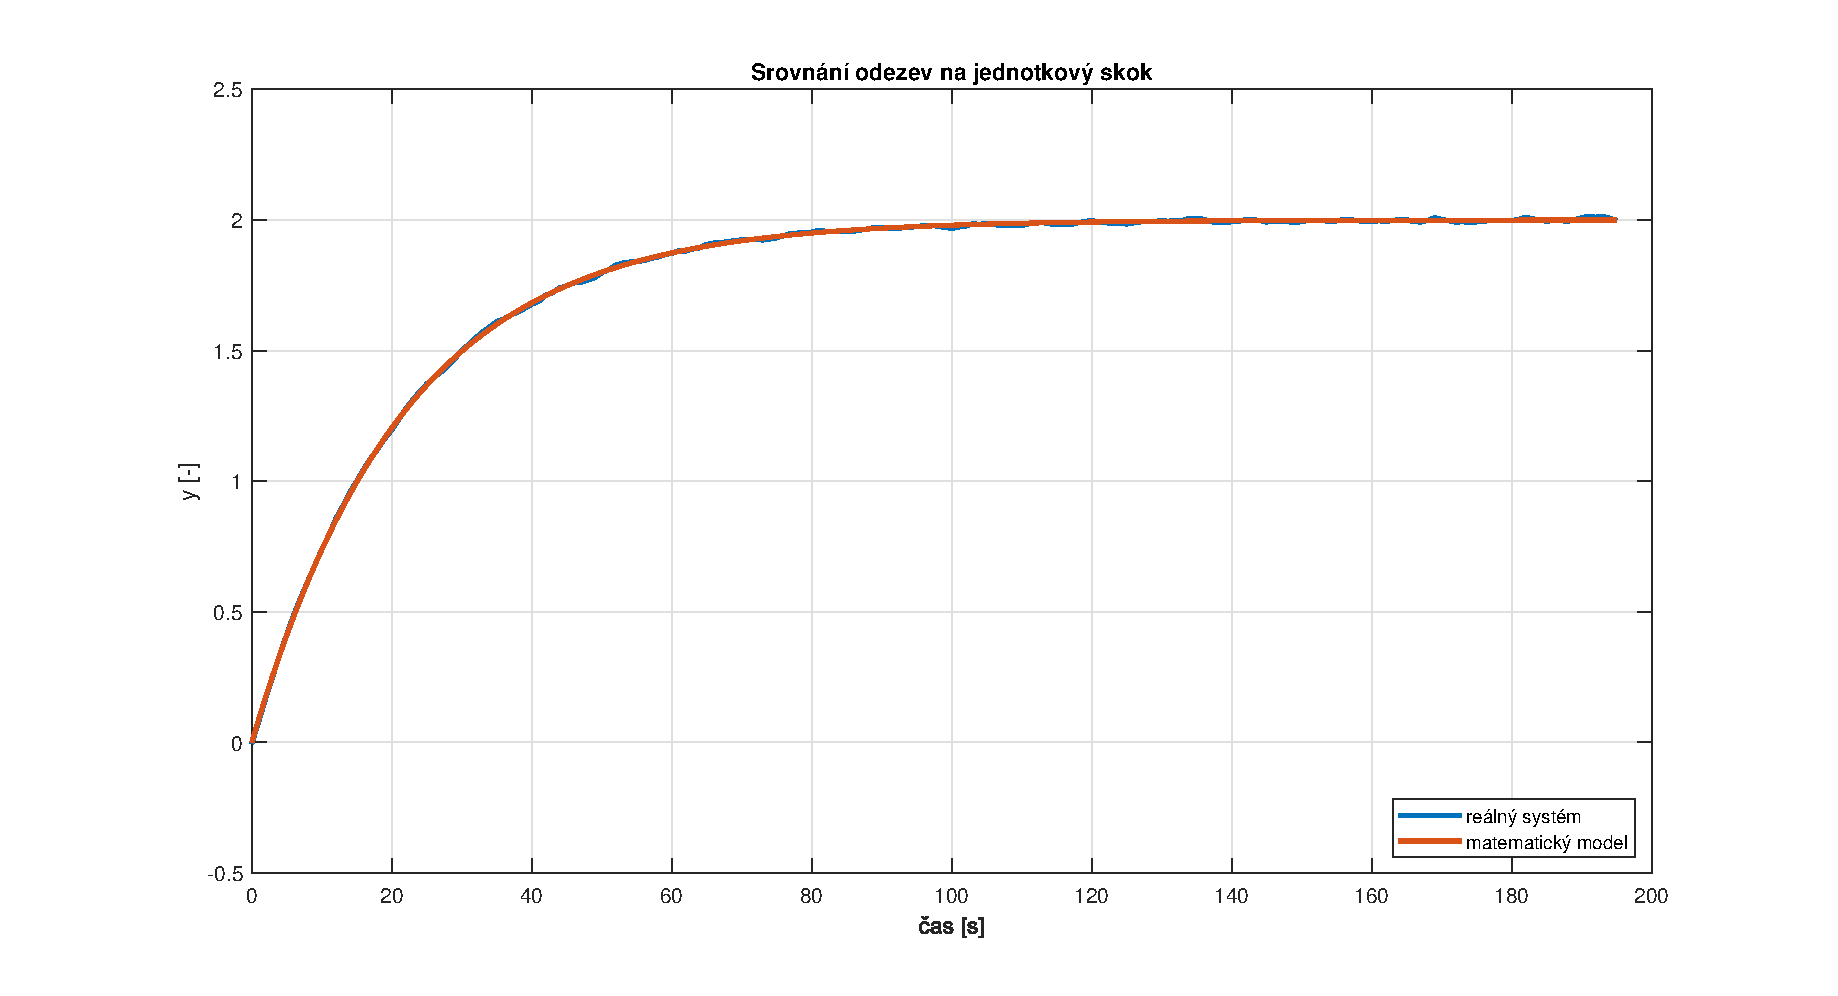
\includegraphics[width=\linewidth]{odezvy1_zaver.eps}
	\caption{Srovnání změřené a simulované odezvy systému prvního řádu}
	\label{fig:zaver1}
\end{figure}

\section{Odezva systému druhého řádu}
Pokuste se identifikovat model druhého řádu. Přenosovou funkci modelu hledejte ve tvaru

\begin{equation}
	F(s) = k \frac{\omega_n^2}{s^2 + 2\zeta \omega_n s + \omega_n^2}.
	\label{eq:obecne2}
\end{equation}
Uveďte ustálenou hodnotu výstupu, překmit a dobu ustálení, dále parametr tlumení $\zeta$,
přirozenou frekvenci $\omega_n$ a zesílení $k$, které jste získali identifikací, a
krátký popis, jak jste při identifikaci postupovali.
Nakonec vložte obrázek obsahující originální odezvu generovanou funkcí a odezvu vámi získaného
matematického modelu.

\textbf{Řešení:} Změřená odezva vykreslená na obrázku \ref{fig:zadani2} je kmitavá. Systém je tedy podtlumený a má pár komplexně sdružených pólů.
Na první pohled lze očekávat nízký koeficient relativního tlumení $\zeta$, neboť exponenciální obálka harmonických kmitů odezvy poklesá velmi pomalu po dobu desítek sekund.
Kvůli nízkému relativnímu tlumení bude pro frekvenci tlumených kmitů platit $\omega_d = \omega_n \cdot \sqrt{1 - \zeta^2} \approx \omega_n$.
\begin{figure}[hbtp]
	\centering
	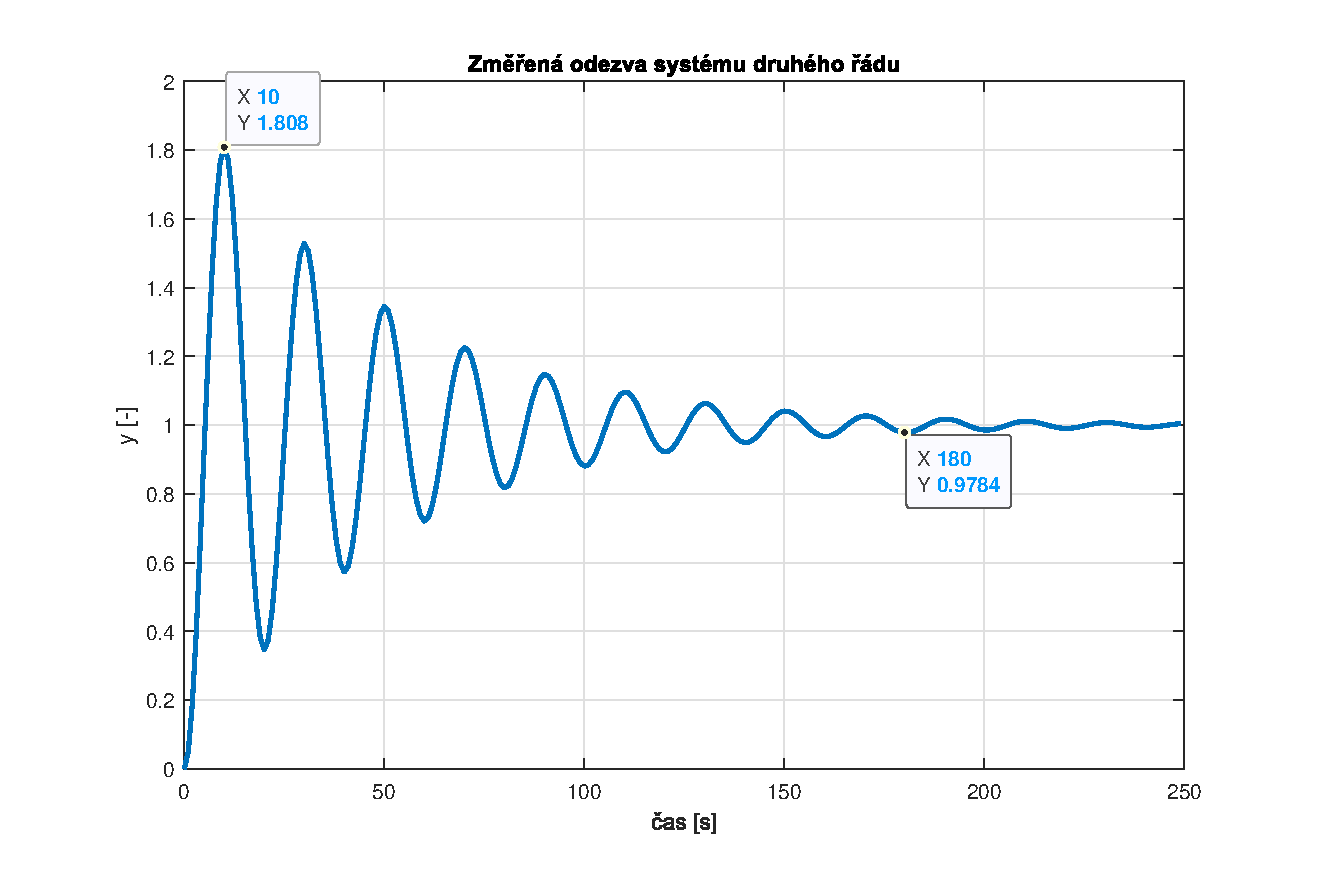
\includegraphics[width=\linewidth]{zadani2.eps}
	\caption{Vygenerovaná odezva systému řádu 2}
	\label{fig:zadani2}
\end{figure}

Pro nekonečný čas se odezva systému asymptoticky ustálí na hodnotě $y = 1$. Protože je zlomek ve vztahu \eqref{eq:obecne2} normovaný na jednotkové statické zesílení,
musí platit $k = 1$. Relativní tlumení $\zeta$ a přirozenou frekvenci oscilací $\omega_n$ lze vypočíst pomocí vztahů s hodnotou překmitu $OS$ a dobou ustálení $T_s$.
Pro podtlumený systém druhého řádu platí
\begin{equation}
	\zeta = \frac{- \ln(OS)}{\sqrt{\pi^2 + \ln^2(OS)}} ~~~~~~~~~ \text{a} ~~~~~~~~~ \omega_n = \frac{4}{T_s \zeta},
	\label{eq:vztahy}
\end{equation}
kde overshoot $OS$ je dán vztahem $OS = \frac{\max y(t) - y(\infty)}{y(\infty)}$.
Z časového průběhu odezvy systému lze odečíst hodnoty $T_s = 180$, $OS = \frac{1.808 - 1}{1} \approx 0.8$.
Po dosazení do \eqref{eq:vztahy} získáme
\begin{equation}
	\begin{split}
		\zeta &= \frac{- \ln(0.8)}{\sqrt{\pi^2 + \ln^2(0.8)}} = 0.071~\text{[-]}\\
		\omega_n &= \frac{4}{180 \cdot 0.071} = 0.313~\text{rad/s}.
	\end{split}
\end{equation}
Dosazením za koeficienty $\zeta$ a $\omega_n$ do \eqref{eq:obecne2} vychází pro přenos identifikovaného systému vztah
\begin{equation}
	F(s) = k \frac{0.313^2}{s^2 + 2 \cdot 0.071 \cdot 0.313 s + 0.313^2} = \frac{0.098}{s^2 + 0.044s + 0.098}.
\end{equation}
Skoková odezva tohoto modelu je na obrázku \ref{fig:zaver2} porovnána se změřenými daty. Typ odezvy je identický,
viditelné jsou drobné deviace v aplitudě odezvy modelu. Ty jsou způsobeny výraznou zaokrouhlovací chybou vnesenou
do výpočtů používáním dvou až tří platných číslic. Nemá však smysl se snažit výpočet zpřesňovat, neboť jeho vstupem
jsou data zatížená nepřesností manuálního odečtení z charakteristiky.
\begin{figure}[hbtp]
	\centering
	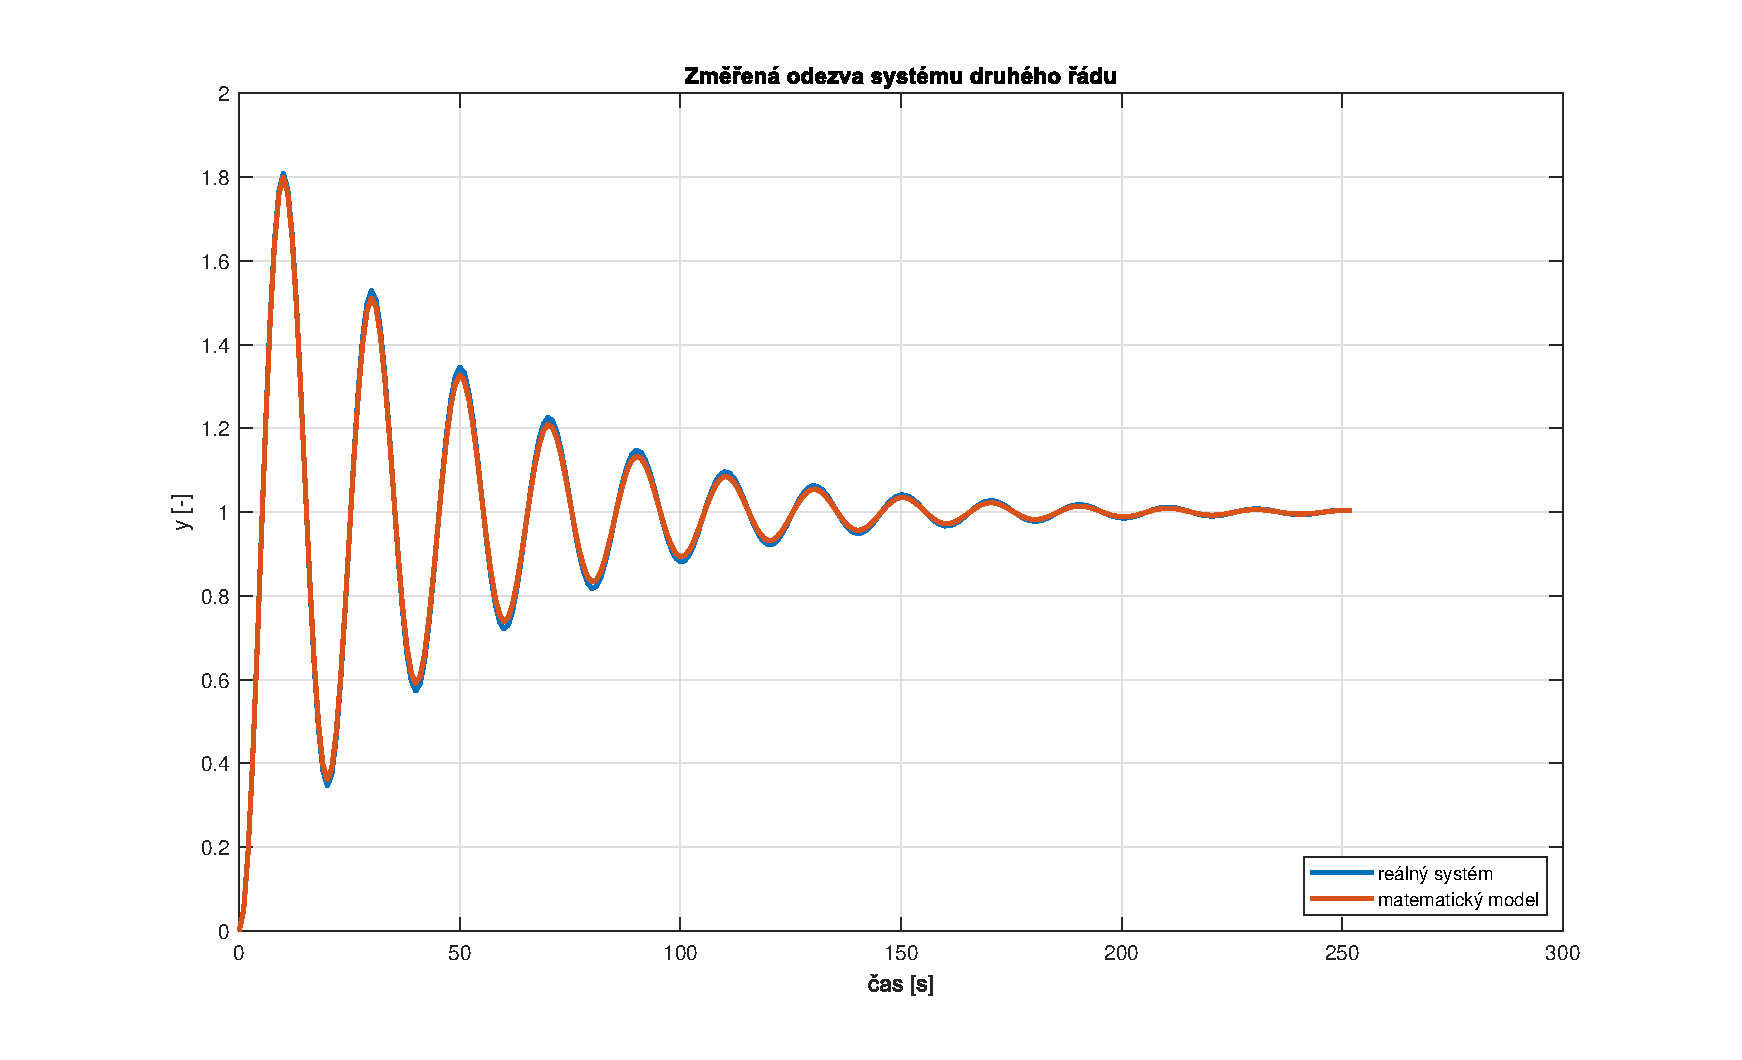
\includegraphics[width=\linewidth]{odezvy2.eps}
	\caption{Srovnání změřené a simulované odezvy systému druhého řádu}
	\label{fig:zaver2}
\end{figure}

\begin{thebibliography}{9}

\bibitem{Wiki}
	\LaTeX tutorials, \url{http://en.wikibooks.org/wiki/LaTeX/}

\bibitem{motivace}
	Gene F. Franklin, \emph{How to balance the LEGO robot in less than 90 seconds} \url{https://www.youtube.com/watch?v=BjDebmqFRuc}

\end{thebibliography}












\end{document}

